\section{Zeitabhängige Probleme}
\label{sec-6}

\subsubsection*{Motivation:}
Anfangs-Randwertprobleme, z.B.\ Wärmeleitung. Suche $u(x,t)$, $x \in \Omega$, $t \in [0,T]$
\begin{align*}
	\partial_t u - \Delta u &= q & & \text{in } \Omega \times (0,T) \\
	u(x,t) &= g_D(x,t) & & \text{auf } \partial\Omega \times (0,T) \\
	u(x,0) &= u_0(x) & & \text{in } \Omega
\end{align*}

\subsubsection*{Numerischer Ansatz:}
Zeitdiskretisierung: Wähle $K \in \N$, $\Delta t := \frac{T}{K}$
\[
	t^k := k \cdot \Delta t, \quad k = 0,\ldots,K
\]
Wähle $X \subseteq Y := L^2(\Omega)$ Lösungsraum bezüglich Ortsraum, z.B.\ $X = L^2(\Omega)$ oder $X = H_0^1(\Omega)$ oder $X = \spn(\mathbbm{1}_{e_i})_{i=1}^{H}$ Finite-Volumen-, oder $X = \spn(\psi_i)_{i=1}^H$ Finite-Elemente-Raum, etc.

Suche Lösungssequenz $u = \seq{u^k}_{k=0}^K \in (X)^{K+1}$ mit $u^k(x) \approx u(x,t^k)$.

Referenzen:
\begin{itemize}
	\item Für PDE-Diskretisierung siehe NUMPDE14/15.
	\item Für Folgende RB-Behandlung siehe auf S.\ 8 genanntes Tutorial.
\end{itemize}

\vspace{10pt}

\begin{bem}
	Statt variationeller Formulierung betrachte im Folgenden operatorbasierte Formulierung, dies erfasst auch Finite-Differenzen oder Finite-Volumen Diskretisierungen.
	Alles Folgende könnte auch durch Variationsformulierung ausgedrückt werden.
\end{bem}

\begin{defn}[Volles Evolutionsproblem $\eprob$]
	Sei $X$ Hilbertraum, $\mu \in \p$: $u(\mu) = \seq{u^k(\mu)}_{k=0}^K \in (X)^{K+1}$ Lösungen von
	\begin{align*}
		\LI^k(\mu) u^{k+1} &= \LE^k(\mu) u^k + b^k(\mu) \\
		u^0 &:= P_X(u_0)
	\end{align*}
	mit $\LI^k$, $\LE^k \in L(X)$, $P_X: Y \to X$ beliebige stetige Projektion.
\end{defn}

\begin{bem} \beginwithlistbem
	\begin{itemize}
		\item Wir verzichten hier wieder auf Ausgabefunktionale.
		\item Obiges erfasst allgemeine implizite/explizite Zeitdiskretisierung wie impliziter/expliziter Euler oder Crank-Nicolson-Verfahren für parabolische oder hyperbolische DGL.
		\item $\LI^k$, $\LE^k$, $b^k$ hängen typischerweise von $\Delta t$ ab.
	\end{itemize}
\end{bem}

\paragraph{Annahmen an Operatoren:}

\begin{itemize}
	\item $\LI^k$, $\LE^k$ seien stetig mit Konstanten $\gamma_I^k(\mu)$, $\gamma_E^k(\mu)$ und uniform in $t$, $\mu$, d.h.\ $\gamma_I^k(\mu) \leq \bar\gamma$, $\gamma_E^k(\mu) \leq \bar\gamma_E$.
	\item $\LI^k$ sei uniform koerziv bzgl.\ $\mu$ und $k$, d.h.\ ex.\ $\bar\alpha_I$, $\alpha_I^k(\mu)$ mit
		\[
			0 < \bar\alpha_I \leq \alpha_I^k(\mu) := \inf_v \frac{\dotp{\LI^k v}{v}_X}{\norm{v}^2}
		\]
	\item $b^k$ seien uniform beschränkt $\norm{b^k(\mu)} \leq \bar\gamma_b$ $\forall k, m$.
	\item $\LI^k$, $\LE^k$ seien separierbar parametrisch mit zeitunabhängigen Komponenten
		\[
			\LI^k(\mu) = \sum_{q=1}^{Q_I} \Theta_{I,q}^k(\mu) \LL_{I,q}, \quad \LL_{I,q} \in L(X)
		\]
		analog für $\LE$, $b^k$, $u_0$.
\end{itemize}

\begin{satz}[Wohlgestelltheit von $\eprob$] \label{6.2}
Die Lösung $u$ von $\eprob$ ist wohldefiniert und beschränkt durch
\begin{align} \label{eq:6.1}
||u^k||_X \leq \Big(\frac{\bar{\gamma_E}}{\bar{\alpha_I}}\Big)^k \cdot ||u^0||_X + \frac{\bar{\gamma_b}}{\bar{\alpha_I}} \sum\limits_{i=0}^{k-1} \Big(\frac{\bar{\gamma_E}}{\bar{\alpha_I}}\Big)^i
\end{align}
\begin{proof}
In Iteration $k$ folgt aus Lax-Milgram Wohldefiniertheit und Schranke
\[
	||u^{k+1}|| \leq \frac{1}{\alpha_I(\mu)} (\gamma_E(\mu)||u^k|| + \gamma_b(\mu))
\]
Schranke (\ref{eq:6.1}) folgt per Induktion

Induktionsanfang:
\[
	||u^0|| \leq \Big(\underbrace{\frac{\bar{\gamma_E}}{\bar{\alpha_I}}}_{=1}\Big)^0 ||u^0|| + \underbrace{\Big(\sum\limits_{i=0}^{-1}(\pdot)^i)}_{=0} \frac{\bar{\gamma_b}}{\bar{\alpha_I}} = ||u^0||
\]
Ind. Schritt:
\begin{align*}
	||u^{k+1}|| \leq \frac{\bar{\gamma_E}}{\alpha_I} ||u^k|| + \frac{\bar{\gamma_b}}{\alpha_I} &\overset{\text{i.A.}}{\leq} \frac{\bar{\gamma_E}}{\alpha_I} \Big((\frac{\bar{\gamma_E}}{\alpha_I})^k ||u^0|| + \frac{\bar{\gamma_b}}{\alpha_I} \sum\limits_{i=0}^{k-1} (\frac{\bar{\gamma_E}}{\alpha_I})^i\Big) + \frac{\bar{\gamma_b}}{\alpha_I} \\
	&=(\frac{\bar{\gamma_E}}{\alpha_I})^{k+1} ||u^0|| + \underbrace{\frac{\bar{\gamma_b}}{\alpha_I} \cdot \sum\limits_{i=1}^{(k+1)-1} (\frac{\bar{\gamma_E}}{\alpha_I})^i + \frac{\bar{\gamma_b}}{\alpha_I}}_{=\frac{\bar{\gamma_b}}{\alpha_I}\cdot \sum\limits_{i=0}^{(k+1)-1}(\dots)}
\end{align*}
\end{proof}
\end{satz}

Man kann zeigen, dass unter geeigneten Voraussetzungen an die Konstanten die rechte Seite von (\ref{eq:6.1}) beschränkt ist für $\Delta t \rightarrow 0$:

\begin{kor}[Beschränkheit uniform in $\Delta t$] \label{6.3}
Sei $\gamma_E \leq 1$, $\alpha_I = 1 + \alpha \delta t$, $\gamma_b = C \cdot \Delta t$. Dann gilt
\[
	\lim\limits_{k \rightarrow \infty} ||u^k|| \leq e^{-\alpha T} ||u^0|| + C \cdot T
\]
\begin{proof}
	\[
		(\frac{\bar{\gamma_E}}{\alpha_I})^k \leq (\frac{1}{1+\alpha \Delta t}^k = (\frac{1}{1+\alpha \frac{T}{k}})^k = (\underbrace{(\frac{1}{1+\frac{\alpha T}{k}})^{\frac{K}{\alpha T}}}_{\rightarrow e^{-1}})^{\alpha T} \rightarrow e^{- \alpha T}
	\]
	\[
		\sum\limits_{i=0}^{k-1} (\frac{\bar{\gamma_E}}{\alpha_I})^i \leq \sum\limits_{i=0}^{k-1} (\frac{1}{1})^i = k
	\]
	\begin{align*}
	\lim\limits_{k \rightarrow \infty} (\text{rechte Seite von  (\ref{eq:6.1})}) &= \lim\limits_{k \rightarrow \infty} (\frac{\bar{\gamma_E}}{\alpha_I})^k ||u^0|| + (\sum\limits_{i=0}^{k-1}(\frac{\bar{\gamma_E}}{\alpha_I})^i)\frac{\bar{\gamma_b}}{\alpha_I} \\
	& \leq e^{- \alpha T} ||u^0|| + \lim\limits_{k \rightarrow \infty} k \cdot \frac{c \cdot \Delta \overbrace{T}^{=\frac{T}{K}}}{1} \\
	&= e^{- \alpha T} ||u^0|| + C \cdot T
	\end{align*}
\end{proof}
\end{kor}

\begin{bem} \beginwithlistbem
	\begin{itemize}
		\item Bedingungen sind für $||\pdot||_X = || \pdot ||_{L^2(\Omega)}$ für FEM/FV/FD Diskretisierungen erfüllbar, also uniforme Beschränktheit in $L^2$-Norm erreichbar.
		\item Falls $|| \pdot ||_X = || \pdot ||_{H^1}$ ist z.\,B. bei FEM $\alpha = \alpha_0 + \alpha \Delta T$ mit $\alpha_0 << 1$ sehr klein $\Rightarrow$ Schranke aus Korollar wächst beliebig für $\Delta t \rightarrow 0$, Schranke also hier nicht sinnvoll, $H^1$ Beschränktheit muss anders geschlossen werden, siehe z.\,B. NUMPDE 14/15.
	\end{itemize}
\end{bem}

\begin{defn}[Reduziertes Evolutionsproblem $\erprob$]
Sei $X_N \subseteq X$ RB-Raum, $\mu \in \p$, $u_N (\mu) = (u_N^k (\mu))_{k=0}^K \in (X_N)^{K+1}$ Lösung von 
\begin{align*}
		\LNI^k(\mu) u_N^{k+1} &= \LNE^k(\mu) u_N^k + b_N^k(\mu) \qquad ,k=0,\dots,K-1 \\
		u_N^0 &= P_{X_N}(P_X(u_0))
\end{align*}
mit
\[
\LNI^k(\mu) := P_{X_N} \circ \LI^k(\mu) \qquad , \qquad \LNE^k(\mu) := P_{X_N} \circ \LE^k(\mu)
\]
\[
	b_N^k(\mu) := P_{X_N} (b^k(\mu))
\]
wobei $P_{X_N}: X \rightarrow X_N$ orthogonale Projektion bzgl. $\dotp{\pdot}{\pdot}_X$.
\end{defn}

\begin{kor}[Wohlgestelltheit \& uniforme Beschränktheit]
Für Lösung $u_N(\mu)$ von $\erprob$ gelten identische Aussaugen aus \ref{6.2} und \ref{6.3} mit identischen Konstanten.
\begin{proof}
Für (\ref{eq:6.1}) analog zu Bew. \ref{6.2} mit $||u_N^0|| = ||P_{X_N}(u^0)|| \leq \underbrace{||P_{X_N}||}_{\leq 1} ||u^0|| \leq ||u^0||$. Konstanten gelten identisch, da Stetigkeit und Koerzivität auf $X_N$ vererbt.
\end{proof}
\end{kor}

\begin{bem}[Regularität bzgl. $\mu$] \beginwithlistbem
	\begin{itemize}
		\item Falls $\Theta_{I,q}^k(\mu)$, etc. Lipschitz-stetig bzgl. $\mu$, so kann man auch Lipschitz-Stetigkeit von $u, u_N$ bzgl. $\mu$ nachweisen.
		\item Falls $\Theta_{I,q}^k(\mu)$ differenzierbar bzgl. $\mu$, so kann man auch Diffbarkeit von $u, u_N$ bzgl. $\mu$ argumentieren mit Hilfe entsprechender Sensitivitätsprobleme. Dies kann in der Parameteroptimierung ausgenutzt werden, siehe z.\,B.
		
		[DH15] Dihlmann \& Haasdonk. ``Certified PDE-constrained parameter optimization using reduced basis surrogate models for evolution problems''. COAP 60: 753-787,2015.
	\end{itemize}
\end{bem}

\begin{satz}[Reproduktion von Lösungen] \label{6.6}
Falls $\{u^k(\mu)\}_{k=0}^K \subset X_N$ so ist $u_N^k(\mu) = u^k(\mu) \,\, , \,\, k=0,\dots,K$.
\begin{proof}
	Per Induktion.
	
	Induktionsanfang: 
	\[
	k=0: \qquad u^0(\mu) \in X_N \Rightarrow u_N^0 = P_{X_N}u^0 = u^0 \text{ weil } P_{X_N}\Big|_{X_N} = \text{Id}
	\]
	
	Induktionsschritt: Sei $u_N^k(\mu) = u^k(\mu)$
	\begin{align*}
		(E_N) &\Rightarrow \LNI^k u_N^{k+1} - \LNE^k u_n^k - b_N = 0 \\
		& \iff P_{X_N}(\LI^k - u_N^{k+1} - \LE^k u_N^k - b^k )= 0
	\end{align*}
	Aus $\eprob$ und I.A. folgt
	\[
		- \LE^k \underbrace{u_N^k}_{=u^k} - b^k = - \LI^k u^{k+1}
	\]
	also $P_{X_N}(\LI^k(u_N^{k+1} - u^{k+1}))=0$
	\begin{align*}
		&\Rightarrow 0 = \dotp{\LI^k(\underbrace{u_N^{k+1}-u^{k+1}}_{\in X_N})}{\underbrace{u_N^{k+1} - u^{k+1}}_{\in X_N}}_X \geq \alpha_I ||u_N^{k+1} - u^{k+1}||^2 \\
		&\Rightarrow ||u_N^{k+1} - u^{k+1}||_X = 0 \Rightarrow u_N^{k+1} = u^{k+1}
	\end{align*}
\end{proof}
\end{satz}

\begin{lemma}[Fehler-Residuums-Beziehung] \label{6.7}
Für $\mu \in \p$ und RB-Lösung $u_N$ definieren wir das Residuum $R^k(\mu) \in X$ durch
\[
	R^k(\mu) := \frac{1}{\Delta t} (\LE^k u_N^k - \LI^k u_N^{k+1} + b^k) \,\, , \,\, k=0,\dots,K-1
\]
Dann erfüllt der Fehler $e^k(\mu) := u^k(\mu) - u_N^k(\mu)$ das Evolutionsproblem
\[
	\LI^k e^{k+1} = \LE^k e^k + \Delta t R^k \,\, , \,\, k=0,\dots,K-1
\]
\begin{proof}
	$\eprob$ und $\erprob$ ergeben
	\begin{align*}
		\LI^k e^{k+1} &= \LI^k u^{k+1} - \LI^k u_N^{k+1} \\
		&= \LE^k u^k + b^k \underbrace{-\LE^k u_N^k + \LE^k u_N^k}_{=0} - \LI^k u_N^{k+1} = \LE^k e^k + \Delta t \cdot R^k
	\end{align*}
\end{proof}
\end{lemma}

Analoge Technik im Bew. zu Satz \ref{6.2} liefert A-posteriori Schranke

\begin{kor}[A-posteriori Fehlerschranke in $X$-Norm] \label{6.8}
Seien $\alpha_{LB}(\mu)$ und $\gamma_{LB}(\mu)$ berechenbare untere/obere Schranken mit
\[
	\gamma_E^k(\mu) \leq \gamma_{UB}(\mu) \leq \bar{\gamma_E} \,\, , \,\, \alpha_I^k(\mu) \geq \alpha_{LB}(\mu) \geq \bar{\alpha_I} \qquad \mu \in \p \,\, , \,\,k=0,\dots,K
\]
Dann gilt für $k=0,\dots,K$:
\[
	||u^k(\mu) - u_N^k(\mu)|| \leq \Delta_N^k(\mu) \text{ mit }
\]
\[
	\Delta_N^k(\mu) := ||e^0||\Big(\frac{\gamma_{UB}(\mu)}{\alpha_{LB}(\mu)}\Big)^k + \frac{\Delta t}{\alpha_{LB}(\mu)} \sum\limits_{i=0}^{k-1}\Big(\frac{\gamma_{UB}(\mu)}{\alpha_{LB}(\mu)}\Big)^{k-i-1} ||R^i||
\]
\begin{proof}
	Analog zu \ref{6.2} liefert Lax Milgram
	\[
		||e^{k+1}|| \leq \frac{\gamma_E^k}{\alpha_I} ||e^k|| + \frac{\Delta t}{\alpha_I} ||R^{k+1}||
	\]
	Per Induktion folgt Beh.
\end{proof}
\end{kor}

\begin{bem} \beginwithlistbem
	\begin{itemize}
		\item Wie in § \ref{sec-3}: Fehler erfüllt $\eprob$ mit Residuum als Inhomogenität, Fehlerschätzer folgt aus Stabilitätsaussage für Fehlergleichung.
		\item Falls $u^0(\mu) \in X_N$ so ist wg. Reproduktion von Lösungen \ref{6.6} $e^0 = 0$, Schranke vereinfacht sich. Dies wird durch $u_q^0 \in X_N$ erreicht.
		\item Residuen-Normen sind wieder Offline/Online-zerlegbar (folgt) also effizient berechenbar.
		\item Fehlerschranke ist meist monoton wachsend in $k$ falls $\alpha_I \leq 1$, während der echte Fehler durchaus fallend sein kann. Daher ist zu erwarten, dass die Effektivitäten $\eta(\mu,t^k) := \frac{\Delta_N^k(\mu)}{||e^k(\mu)||_X}$ mit wachsendem $k$ schlechter werden:
\begin{figure}[H]
  \centering\small
    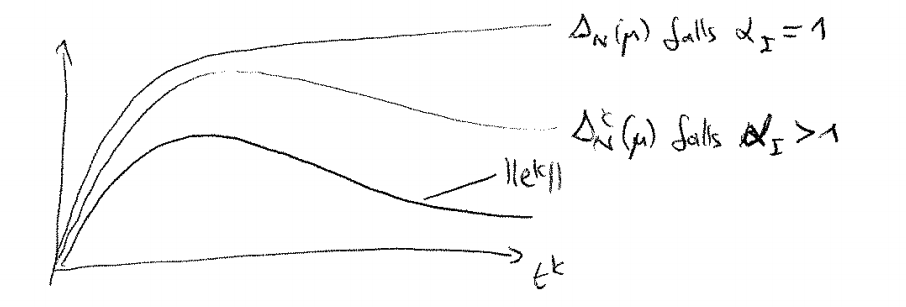
\includegraphics[width = 0.8 \textwidth]{Bilder/Effektivitätsverläufe.png}
  \label{fig:Effektivitätsverläufe}
\end{figure}
Falls $\alpha_I > 1$, können Fehlerschätzer auch fallend sein.
		\item Beschränktheit uniform in $\Delta t$: Unter Vorauss. von Korollar \ref{6.3} und Annahme, dass $||R^k|| \leq C \,\, \forall \, k, \Delta t$, so bleibt $\Delta_N$ für $\Delta t \rightarrow 0$ beschränkt.
	\end{itemize}
\end{bem}

\paragraph*{Offline-/Online-Zerlegung}

\begin{itemize}
	\item Diskrete Formulierung von $\eprob$:
	
	Sei $\Psi := \{\psi_i\}_{i=1}^H$ Basis von $X$, $\underline{K}:= \Big(\dotp{\psi_i}{\psi_j} \Big)_{i,j=1}^H$
	
	Sei $\underline{L}_I^k \in \R^{H \times H}$ so dass für alle $v, v' \in X$ und deren Koeff.-Vektoren $\underline{v}, \underline{v'} \in \R^H$ gilt
	\[
		v' = \LI^k v \iff \underline{v'} = \underline{L}_I^k \underline{v}
	\]
	analog $\underline{L}_E^k \in \R^{H \times H}$, sei $\underline{b}^k \in \R^H$ Koeff.-Vektor von $b^k \in X$.
	
	Bestimme $\underline{u}(\mu) = (\underline{u}^k(\mu))_{k=0}^K \in (\R^H)^{K+1}$ Koeffizientenvektoren von $u(\mu)$ via
	\begin{align*}
		\underline{u}^0 \text{ Koeff.-Vektor von } u^0 = P_X(u_0) \\
		\underline{L}_I^k \underline{u}^{k+1} = \underline{L}_E^k \underline{u}^k + \underline{b}^k \qquad k=0,\dots,K-1
	\end{align*}
	\item Diskrete Form von $\erprob$
	
	Sei $\Phi_N = \{\phi_1,\dots,\phi_N\} \subset X$ Basis von $X_N$, $\underline{\phi}_n \in \R^H$ zugehörige Koeff.-Vektoren, $\underline{\Phi}_N = (\underline{\phi}_1,\dots,\underline{\phi}_N)$
	
	Bestimme $(\underline{u}_N^k(\mu))_{k=0}^K \in (\R^N)^{K+1}$ Koeff.-Vektor von $u_N(\mu)$ bzgl. $\Phi_N$:
	\begin{align}
	u_N^0 := P_{X_N} u^0 &\iff u_N^0 \in X_N: \,\, \dotp{u_N^0}{\phi_i}_X = \dotp{u^0}{\phi_i}_X \,\, i=1,\dots,N \notag \\
	&\iff \underline{K}_N \underline{u}_N^0 = (\dotp{u^0}{\phi_i}_X)_{i=1}^N \text{ mit } \underline{K}_N := (\dotp{\phi_i}{\phi_j})_{i,j=1}^N  \label{eq:6.2}\\
	\underline{L}_{N,I}^k \underline{u}_N^{k+1} = \underline{L}_{N,E} \underline{u}_N^k + \underline{b}_N^k \label{eq:6.3}
	\end{align}
	mit $(\underline{L}_{N,I}^k)_{i,j} :=\dotp{\LI^k \phi_j}{\phi_i}_X = \underline{\phi}_i^T \underline{K} \underline{L}_I^k \underline{\phi}_j$, analog für $\underline{L}_{N,E}^k$
	
	$(\underline{b}_N^k)_i := \dotp{b^k}{\phi_i}_X = \underline{\phi}_i^T \underline{K} \underline{b}^k$ also
	\begin{align} \label{eq:6.4}
	L_{N,I}^k := \underline{\Phi}_N^T \underline{K} \underline{L}_I^k \underline{\Phi}_N, b_N^k := \underline{\Phi}_N^T \underline{K} \underline{b}^k
	\end{align}
	\item Offline-/Online-Zerlegung dann mit parametersep. klar:
	
	Offline: hochdimensionale Daten: $\underline{\Phi}_N, \underline{K}$
	niedrigdimensionale Daten: $\underline{K}_N$, Komponenten $\underline{u}_N^{0,q}$ analog zu (\ref{eq:6.2}), $\underline{L}_{N,I,q}, \underline{L}_{N,E,q}, \underline{b}_{N,q}$ analog zu (\ref{eq:6.4}).
	
	Online: Auswerten von $\Theta_{E,q}^k(\mu), \Theta_{I,q}^k(\mu), \Theta_{b,q}^k(\mu), \Theta_{k_0,q}(\mu)$. Assemblieren und Lösen von (\ref{eq:6.3}).
	\item Diskrete Form der Residuen-Norm aus Satz \ref{6.8}:
	\begin{align*}
	||R^{k+1}||^2 &= \dotp{\frac{1}{\Delta t}(\LE^k u_N^k - \LI^k u_N^{k+1} + b^k)}{\frac{1}{\Delta t}(\LE^k u_N^k - \LI^k u_N^{k+1} + b^k)}_X \\
	&= \frac{1}{\Delta t^2} \big((\underline{u}_N^k)^T \underline{M}_{EE}^k \underline{u}_N^k + (\underline{u}_N^{k+1})^T \underline{M}_{II}^k \underline{u}_N^{k+1} + \underline{M}_{bb} \\ &- 2 (\underline{u}_N^k)^T \underline{M}_{EI} \underline{u}_N^{k+1} + 2 (\underline{u}_N^k)^T \underline{M}_{Eb} - 2 (\underline{u}_N^{k+1})^T\underline{M}_{IB}\big)
	\end{align*}
	Mit $\underline{M}_{EE}^k := (\dotp{\LE^k \phi_i}{\LE^k \phi_j}_X)_{i,j=1}^N = \underline{\Phi}_N^T (\underline{L}_E^k)^T \underline{K} \underline{L}_E^k \underline{\Phi}_N \,\, \in \R^{N \times N}$ analog $\underline{M}_{II}^k, \underline{M}_{EI}^k \,\, \in \R^{N \times N}$ und $\underline{M}_{Eb}^k := (\dotp{b^k}{\LE^k \phi_i}_X)_{i=1}^N = \big((\underline{b}^k)^T \underline{K} \underline{L}_E^k \underline{\Phi}_N \big)^T \,\, \in \R^N$, analog $\underline{M}_{Ib}^k$ und $\underline{M}_{bb} := \dotp{b^k}{b^k}_X \,\, \in \R$
	\item Separierbare Param-abh. ``vererbt'': $M_{(\ast)(\ast \ast)}$ separierbar mit $Q_{(\ast)}Q_{(\ast \ast)} =: Q_{(\ast)(\ast \ast)}:$
	\[
	\underline{M}_{EE}^k = \sum\limits_{q,q'=1}^{Q_E} \underbrace{\Theta_{E,q}^k(\mu)\Theta_{E,q'}^k(\mu)}_{\Theta_{EE}^{q,q'}(\mu,k} \underbrace{\underline{\Phi}_N^T(\underline{L}_{E,q})^T \underline{K} \underline{L}_{E,q'} \underline{\Phi}_N}_{\underline{M}_{EE}^{q,q'}}
	\]
	Damit Offline-/Online Zerlegung klar.
\end{itemize}

\begin{bem}[Umgehen von $\underline{L}_E^k, \underline{L}_I^k, \underline{b}^k$ bei FEM] 
Jedes Evolutionsschema $\eprob$ lässt sich diskret schreiben als
	\begin{align}\label{eq:6.5}
	\underline{L}_I^k \underline{u}^{k+1} = \underline{L}_E^k \underline{u}^k + \underline{b}^k
	\end{align}
	Dies ist aber nur bei FD/FV auch tatsächlich die Berechnungsvorschrift. Bei FEM liegt $\underline{L}_E^k, \underline{L}_I^k, \underline{b}^k$ nicht vor. Man löst stattdessen
	\begin{align} \label{eq:6.6}
	\underline{\tilde{L}}_I^k \underline{u}^{k+1} = \underline{\tilde{L}}_E^k \underline{u}^k + \underline{\tilde{b}}^k
	\end{align}
	z.\,B. Wärmeleitung mit $g_0 = 0$; impliziter Euler:
	\begin{align*}
	&\int\limits_{\Omega} \frac{u^{k+1}- u^k}{\Delta t} v + \int\limits_{\Omega} \nabla u^{k+1} \cdot \nabla v = \int\limits_{\Omega} q v \qquad \forall \,\, v \in X = H_0^1(\Omega) \\
		\iff \qquad &\underbrace{\int\limits_{\Omega} u^{k+1} v + \Delta t \nabla u^{k+1} \cdot \nabla v}_{:= \dotp{\LI^k u^{k+1}}{v}_X} = \underbrace{\int\limits_{\Omega} u^k v}_{:= \dotp{\LE^k u^k}{v}_X} + \underbrace{\Delta t \int\limits_{\Omega} q v}_{\dotp{b^k}{v}_X}
	\end{align*}
	mit geeigneten Riesz-Repr. $\LI^k u^{k+1}, \LE^k u^{k+1}, b^k \in X$.
	D.\,h. in (\ref{eq:6.6}) lauten Matrizen
	\[
		(\underline{\tilde{L}}_I^k)_{i,j} = \int\limits_{\Omega} \psi_i \psi_j + \Delta t \nabla \psi_i \cdot \nabla \psi_j \,\, , \text{ etc.}
	\]
	Beziehung zu (\ref{eq:6.5}) ergibt sich leicht
	\[
	(\underline{\tilde{L}}_I^k)_{ij} \overset{\text{sym.}}{=} \dotp{\LI^k \psi_j}{\psi_i}_X = \dotp{\psi_i}{\LI^k \psi_j} = e_i^T \underline{K} \underline{L}_I^k e_j = (\underline{K} \underline{L}_I^k)_{ij}
	\]
	analog für $\underline{\tilde{L}}_E^k, \underline{\tilde{b}}^k$. FEM Diskretisierung löst also faktisch
	\[
		\underline{K} \underline{L}_I^k \underline{u}^{k+1} = \underline{K} \underline{L}_E^k \underline{u}^k + \underline{K} \underline{b}^k
	\]
	mit identischer Lösung wie (\ref{eq:6.5}).
	
	Man erspart sich die teure Berechnung von $\underline{L}_I^k = K^{-1} \underline{\tilde{L}}_I^k$, etc. In Offline-Online-Zerlegung kann man $\underline{L}_I^k$, etc. auch umgehen und nur mit $\underline{\tilde{L}}_I^k$ und wenigen weiteren Riesz-Repräsentanten arbeiten.
\end{bem}

\paragraph*{Numerisches Beispiel} demos\_chapter6(1): RB-Schritte mit convdiff\_model, eine instationäre Konvektions-Diffusions-Gleichung mit FV Diskretisierung.

\subsection{Raum-Zeit-Betrachtung}

\begin{itemize}
	\item In NUMPDE14/15 wird für Wärmeleitung ein Stabilitätsergebnis in einer Raum-Zeit-Energienorm formuliert. Diese Technik liefert einen Fehlerschätzer in Raum-Zeit-Energienorm.
	\item Weitere Forderung an Operatoren:
		\begin{description}
	\item $\LE^k$ unabhängig von $\Delta t, k$, $\Leins := \LE^k$ (z.\,B. rein implizite Diskretisierung)
	\item $\Leins$ selbstadjungiert $\dotp{\Leins u}{v}_X = \dotp{u}{\Leins v}_X$ und positiv definit.
	\item $\LI^k = \Leins + \Delta t \Lzwei$ mit $\Lzwei$ stetig, koerziv mit Konstante $\alpha$, unabhängig von $\Delta t$
	\item $\Lzwei$ selbstadjungiert 
		\end{description}
\end{itemize}

\begin{defn}[Raum-Zeit-Energienorm]
Definiere Raum-Zeit-Energienorm $|||\pdot|||_{\mu}$ auf $(X)^k$ durch:
\[
|||u(\mu)|||_{\mu} := |||(u^k)_{k=1}^K|||_{\mu} := \Big(\dotp{\Leins u^k}{u^k}_X + \Delta t \sum\limits_{k=1}^K \dotp{\Lzwei u^k}{u^k}_X \Big)^{\frac{1}{2}}
\]
\end{defn}

\begin{lemma}[Young'sche Ungleichung]
Für alle $a, b, \epsilon \in \R$ gilt
\[
	a b \leq \frac{1}{2 \epsilon^2} a^2 + \frac{1}{2} \epsilon^2 b^2
\]
\begin{proof}
	$ 0 \leq (\frac{a}{\epsilon}- \epsilon b)^2 = \frac{a^2}{\epsilon^2} - 2 \frac{a}{\epsilon} \epsilon b + \epsilon^2 b^2 \Rightarrow$ Beh.
\end{proof}
\end{lemma}

\begin{satz}[A-posteriori Fehlerschätzer Raum-Zeit-Energienorm]
$\forall \mu \in \p, u(\mu), u_N(\mu)$ Lösung von $\eprob, \erprob$ gilt:
\[
	|||u(\mu) - u_N(\mu)|||_{\mu} \leq \Delta_N^{en}(\mu) := (\frac{\Delta t}{\alpha} \sum\limits_{i=1}^K ||R^k||^2 + \dotp{\Leins e^0}{e^0}_X)^{\frac{1}{2}}
\]
\begin{proof}
Fehler Residuums-Gleichung aus \ref{6.7}:
\[
	\LI^k e^{k+1} = \LE^k e^k + \Delta t R^{k+1}
\]
Additive Zerlegung und Skalarprodukt mit $e^{k+1}$:
\[
\dotp{\Leins e^{k+1}}{e^{k+1}} + \Delta t \dotp{\Lzwei e^{k+1}}{e^{k+1}}_X = \underbrace{\dotp{\Leins e^k}{e^{k+1}}}_{:= T_1} + \Delta t \underbrace{\dotp{R^{k+1}}{e^{k+1}}_X}_{:=T_2}
\]
\begin{align*}
T_1 &\overset{\text{CS bzgl } \dotp{\Leins \pdot}{\pdot}}{\leq} \big(\dotp{\Leins e^k}{e^k}_X \big)^{\frac{1}{2}} \big(\dotp{\Leins e^{k+1}}{e^{k+1}}_X \big)^{\frac{1}{2}} \\
&\overset{\text{Young, } \epsilon=1}{\leq} \frac{1}{2} \dotp{\Leins e^k}{e^k}_X + \frac{1}{2} \dotp{\Leins e^{k+1}}{e^{k+1}}_X \\
T_2 &\leq ||R^{k+1}|| ||e^{k+1}|| \overset{\text{Young, } \epsilon^2 = \alpha}{\leq} \frac{1}{2 \alpha} ||R^{k+1}||^2 + \frac{1}{2} \underbrace{\alpha ||e^{k+1}||^2}_{\leq \dotp{\Lzwei e^{k+1}}{e^{k+1}}}
\end{align*}
Damit
\[
	\frac{1}{2} \dotp{\Leins e^{k+1}}{e^{k+1}} - \frac{1}{2} \dotp{\Leins e^{k}}{e^{k}} + \frac{1}{2} \Delta t \dotp{\Lzwei e^{k+1}}{e^{k+1}} \leq \Delta t \frac{1}{2 \alpha} ||R^{k+1}||^2
\]
Summe über $k=0,\dots,K-1$ Teleskopsumme:
\[
	\frac{1}{2} \dotp{\Leins e^{0}}{e^{0}} - \frac{1}{2} \dotp{\Leins e^{0}}{e^{0}} + \frac{1}{2} \Delta t \sum\limits_{k=1}^K \dotp{\Lzwei e^{k}}{e^{k}} \leq \sum\limits_{k=1}^K \frac{\Delta t}{2 \alpha} ||R^{k}||^2
\]
\[
	\underbrace{\dotp{\Leins e^{k}}{e^{k}} + \Delta t \sum\limits_{k=1}^K \dotp{\Lzwei e^{k}}{e^{k}}}_{|||e|||_{\mu}^2} \leq \dotp{\Leins e^{0}}{e^{0}} + \sum\limits_{k=1}^K \frac{\Delta t}{\alpha} ||R^{k}||^2
\]
\end{proof}
\end{satz}

\begin{bem} \beginwithlistbem
\begin{itemize}
	\item Energie-Norm FS haben praktisch bessere Effektivitäten als $X$-Norm-FS.
	\item Erweiterungen existieren:
	\begin{itemize}
		\item $\LI$ darf nicht-koerziv sein: Knezevic \& Patera, SIAM J. Scientific Comp. 2010
		\item $Y=X=L^2(\Omega)$, $\LE$ darf $\Delta t$-abhängig sein: Haasdonk \& Ohlberger, M2AN, 2008
	\end{itemize}
	\item Durch Interpretation von $\eprob$ als ein Petrov-Galerkin Verfahren kann man ganz allgemeine Fehlerschranken und Effektivitätsschranken aus §\ref{sec-4} folgen:
\end{itemize}
\end{bem}

\begin{kor}[Evolutionsschema als Raum-Zeit-Petrov-Galerkin-Verfahren] \label{6.12}
Sei $X_1 := X_2 := (X)^{k+1}$ mit Skalarprodukt $\dotp{\pdot}{\pdot}_{X_1}, \dotp{\pdot}{\pdot}_{X_2}$ $X_{N,1} \subset X_1, X_{N,2} \subset X_2$ mit $\dim(X_{N,1}) = \dim(X_{N,2})$.

Wir definieren param. (Bi-)Linearform:
\begin{align*}
a(u,v;\mu) &:= \sum\limits_{k=0}^{K-1} \dotp{\LI^k u^{k+1} - \LE^k u^k}{v^{k+1}}_X + \dotp{u^0}{v^0}_X & \forall \,\, (u,v) \in X_1 \times X_2 \\
f(v;\mu) &:= \sum\limits_{k=0}^{K-1} \dotp{b^k}{v^{k+1}}_X + \dotp{P_X u_0}{v^0}_X & \forall \,\, v \in X_2
\end{align*}
Dann sind $\eprob$, $\erprob$ äquivalent zu $\prob$, $\rprob$ aus §\ref{sec-4}, d.\,h.
\begin{align*}
&u(\mu) \in X_1: &a(u(\mu),v;\mu) = f(v;\mu) &\forall \,\, v \in X_2 \\
&u_N(\mu) \in X_{N,1}: &a(u_N(\mu),v;\mu) = f(v;\mu) &\forall \,\, v \in X_{N,2} \\
\end{align*}
Wegen Wohlgestelltheit von $\eprob$, $\erprob$ ex. info-sup Konstante $\beta_N(\mu) > 0$ und 
\[
||u(\mu) - u_N(\mu)||_{X_1} \leq \frac{||v_r||_{X_2}}{\beta_N(\mu)} =: \Delta_N(\mu)
\]
mit $v_r \in X_2$ Riesz-Repr. des Residuums, d.\,h. $\dotp{v_r}{v}_{X_2} = f(v) - a(u_N,v), v \in X_2$. Mit $\gamma_a(\mu) > 0$ Stetigkeitskonstante von $a(\pdot,\pdot;\mu)$ gilt Effektivitätsschranke
\[
	\frac{\Delta_N(\mu)}{||u(\mu) - u_N(\mu)||_{X_1}} \leq \frac{\gamma_a(\mu)}{\beta_N(\mu)} 
\]
\end{kor}

\begin{bem} \beginwithlistbem
	\begin{itemize}
		\item Diese Raum-Zeit Interpretation ist eine zeit-diskrete Variante einer kontinuierlichen Formulierung aus Urban \& Patera, CRAS, 2012
		\item \ref{6.12} ist sehr allgemein, erlaubt beliebige Wahl der Skalarprodukte
	\end{itemize}
\end{bem}

\subsection{Basisgenerierung mit POD-Greedy-Verfahren}

\paragraph*{Motivation}

\begin{itemize}
	\item Lösungsmannigfaltigkeit $\{u(\mu,t)| \mu \in \p, t\in [0,T]\}$ hat Dimension $p+1$
	\item Kausalität: $u^{k+1}(\mu)$ hängt von $u^k(\mu)$ ab. Man kann nicht $u^{k+1}(\mu)$ berechnen, ohne vorher $u^k(\mu)$ zu bestimmen.
	\item Approximation: $u^k \in X_N$ ist nicht hinreichend für $u_N^k = u^k$. Nach \ref{6.6} ist $\{u^k\}_{k=0}^K \subset X_N$ erforderlich, also gesamte Trajektorie muss gut approximiert werden.
	
	$\Rightarrow$ Trajektorien-Orientierung: Ziele auf gute Trajektorien-Approx. statt einzelne Snapshots. Benutze alle Snapshots einer Trajektorie um teure Rechenergebnisse optimal auszunutzen.
	
	Ansatz: suche
	\[
		X_N \approx \op{argmin}\limits_{\substack{Y \subset X \\ \dim Y =N}} \sup\limits_{\mu \in \p} \frac{1}{(k+1)} \sum\limits_{k=0}^K ||u^k(\mu) - P_Y u^k(\mu)||^2
	\]
	Approximation durch endliches $\p_{train}$, ``Greedy'' bzgl. $\mu$, POD bzgl. $k$:
\end{itemize}

\begin{defn}[POD-Greedy-Verfahren]
Sei $\p_{train} \subseteq \p, \epsilon_{tol} > 0, \Phi_{N_0} \subset X$ ONB, $N_0 := |\Phi_{N,0}$ gegeben, $\Delta(\mu,Y)$ ein Fehlerindikator.

Setze $N:= N_0$, $X_N :0 \op{span}(\Phi_N)$
\begin{align*}
\text{Solange } &\epsilon_N := \max\limits_{\mu \in \p_{train}} \Delta(\mu,X_N) > \epsilon_{tol} \\
&\mu_{N+1} := \op{argmax}\limits_{\mu \in \p_{train}} \Delta(\mu,X_N) \\
&\text{Berechne Trajektorie } \{u^k(\mu_{N+1})\}_{k=0}^K \\
&\text{Berechne Projektionsfehler-Trajektorie } e_{N+1}^k := u^k(\mu_{N+1}) - P_{Y_N}u^k(\mu_{N+1}) \\
&\text{Bestimme neuen Basisvektor durch POD: } \phi_{N+1} := POD_1 (\{e_{N+1}^k\}_{k=0}^K) \\
&\text{Erweitere Basis und Raum } \Phi_{N+1} := \Phi_N \cup \{\phi_{N+1}\}, X_{N+1} := \op{span} \Phi_{N+1} \\
&N := N+1
\end{align*}
\end{defn}

\begin{bem} \beginwithlistbem
	\begin{itemize}
		\item $\phi_{N+1}$ erhält ``maximale \emph{neue} Information'' durch Berechnung von $\{e_{N+1}^k\}_{k=0}^K$
		\item Im Gegensatz zu normalem Greedy aus §\ref{sec-3} können hier Parameter mehrmals ausgewählt werden, denn mit einer Mode ist nicht die gesamte Trajektorie exakt approximiert.
		\item Man kann mit $\Phi_{N_0} = \emptyset$ beginnen, aber es ist vorteilhaft, $u^0$-Komponenten als Startbasis zu wählen: $X_{N_0} := \op{span}(u^{0,q})_{q=1}^{Q_{u_0}}$. Damit ist Anfangsfehler im $0$ und Term in Fehlerschätzer entfällt.
		\item POD-Greedy liefert ONB nach Konstruktion
		\item Verfahren wurde erstmals in Haasdonk \& Ohlberger, M2AN, 2008 vorgestellt, ist seither Standard in zeitabhängigen RB-Problemen
		\item Man kann wieder Konvergenzraten beweisen Haasdonk, M2AN, 2012
	\end{itemize}
\end{bem}

\paragraph*{Numerisches Beispiel} demos\_chapter6(2): POD-Greedy-Basis Illustration

\begin{itemize}
	\item Anfangsdaten-Komponenten, danach Moden
	\item ``exponentieller'' Abfall des Fehlerschätzers
	\item mehrfache Auswahl der Paramter
	\item Overfitting bei kleiner Trainingsmenge
\end{itemize}
